\documentclass[11pt,a4paper,titlepage]{article}
\usepackage[a4paper]{geometry}
\usepackage[utf8]{inputenc}
\usepackage[english]{babel}
\usepackage{lipsum}
\usepackage{eurosym}

\usepackage{amsmath, amssymb, amsfonts, amsthm, mathtools}
% mathtools for: Aboxed (put box on last equation in align envirenment)
\usepackage{microtype} %improves the spacing between words and letters

\usepackage{lipsum}
\usepackage{threeparttable}
\usepackage{tabularx}
\usepackage{multirow}
\usepackage{booktabs}
\newcommand{\tabitem}{~~\llap{\textbullet}~~}
\usepackage{graphicx}
\graphicspath{ {./pics/} {./eps/}}
\usepackage{epsfig}
\usepackage{epstopdf}
%%%%%%%%%%%%%%%%%%%%
%Figures
%%%%%%%%%%%%%%%%%%%%
\graphicspath{{./figures/}}
%%%%%%%%%%%%%%%%%%%%%%%%%%%%%%%%%%%%%%%%%%%%%%%%%%
%% COLOR DEFINITIONS
%%%%%%%%%%%%%%%%%%%%%%%%%%%%%%%%%%%%%%%%%%%%%%%%%%
\usepackage[dvipsnames]{xcolor} % Enabling mixing colors and color's call by 'svgnames'
%%%%%%%%%%%%%%%%%%%%%%%%%%%%%%%%%%%%%%%%%%%%%%%%%%
\definecolor{MyColor1}{rgb}{0.2,0.4,0.6} %mix personal color
\newcommand{\textb}{\color{Black} \usefont{OT1}{lmss}{m}{n}}
\newcommand{\blue}{\color{MyColor1} \usefont{OT1}{lmss}{m}{n}}
\newcommand{\blueb}{\color{MyColor1} \usefont{OT1}{lmss}{b}{n}}
\newcommand{\red}{\color{LightCoral} \usefont{OT1}{lmss}{m}{n}}
\newcommand{\green}{\color{Turquoise} \usefont{OT1}{lmss}{m}{n}}
%%%%%%%%%%%%%%%%%%%%%%%%%%%%%%%%%%%%%%%%%%%%%%%%%%


%%%%%%%%%%%%%%%%%%%%%%%%%%%%%%%%%%%%%%%%%%%%%%%%%%
%% FONTS AND COLORS
%%%%%%%%%%%%%%%%%%%%%%%%%%%%%%%%%%%%%%%%%%%%%%%%%%
%    SECTIONS
%%%%%%%%%%%%%%%%%%%%%%%%%%%%%%%%%%%%%%%%%%%%%%%%%%
\usepackage{titlesec}
\usepackage{sectsty}
%%%%%%%%%%%%%%%%%%%%%%%%
%set section/subsections HEADINGS font and color
\sectionfont{\color{MyColor1}}  % sets colour of sections
\subsectionfont{\color{MyColor1}}  % sets colour of sections

%set section enumerator to arabic number (see footnotes markings alternatives)
\renewcommand\thesection{\arabic{section}.} %define sections numbering
\renewcommand\thesubsection{\thesection\arabic{subsection}} %subsec.num.

%define new section style
\newcommand{\mysection}{
\titleformat{\section} [runin] {\usefont{OT1}{lmss}{b}{n}\color{MyColor1}}
{\thesection} {3pt} {} }

%%%%%%%%%%%%%%%%%%%%%%%%%%%%%%%%%%%%%%%%%%%%%%%%%%
%		CAPTIONS
%%%%%%%%%%%%%%%%%%%%%%%%%%%%%%%%%%%%%%%%%%%%%%%%%%
\usepackage{caption}
\usepackage{subcaption}
%%%%%%%%%%%%%%%%%%%%%%%%
\captionsetup[figure]{labelfont={color=Turquoise}}

%%%%%%%%%%%%%%%%%%%%%%%%%%%%%%%%%%%%%%%%%%%%%%%%%%
%		!!!EQUATION (ARRAY) --> USING ALIGN INSTEAD
%%%%%%%%%%%%%%%%%%%%%%%%%%%%%%%%%%%%%%%%%%%%%%%%%%
%using amsmath package to redefine eq. numeration (1.1, 1.2, ...)
%%%%%%%%%%%%%%%%%%%%%%%%
\renewcommand{\theequation}{\thesection\arabic{equation}}

%set box background to grey in align environment
\usepackage{etoolbox}% http://ctan.org/pkg/etoolbox
\makeatletter
\patchcmd{\@Aboxed}{\boxed{#1#2}}{\colorbox{black!15}{$#1#2$}}{}{}%
\patchcmd{\@boxed}{\boxed{#1#2}}{\colorbox{black!15}{$#1#2$}}{}{}%
\makeatother
%%%%%%%%%%%%%%%%%%%%%%%%%%%%%%%%%%%%%%%%%%%%%%%%%%

\newcommand{\DP}[1]{\textcolor{blue}{\textbf{(DP says: #1)}}}
\newcommand{\cri}[1]{\textcolor{yellow}{\textbf{(Cri says: #1)}}}

\makeatletter
\let\reftagform@=\tagform@
\def\tagform@#1{\maketag@@@{(\ignorespaces\textcolor{red}{#1}\unskip\@@italiccorr)}}
\renewcommand{\eqref}[1]{\textup{\reftagform@{\ref{#1}}}}
\makeatother
\usepackage[hidelinks]{hyperref}

%% LISTS CONFIGURATION %%
\usepackage{enumitem}
\setlist[enumerate,1]{start=0}
\renewcommand{\labelenumii}{\theenumii}
\renewcommand{\theenumii}{\theenumi.\arabic{enumii}.}

%%%%%%%%%%%%%%%%%%%%%%%%%%%%%%%%%%%%%%%%%%%%%%%%%%
%% PREPARE TITLE
%%%%%%%%%%%%%%%%%%%%%%%%%%%%%%%%%%%%%%%%%%%%%%%%%%
\title{\blue Satellite Communications \\
\blueb Satellite system to provide communication services to polar regions in Europe and Russia}
\author{Ana Reviejo Jiménez \\ Marta Munilla Díez\\ Oscar Pla Terrada\\ Davide Peron\\ Cristina Gava\\ Javier Garcia Camin}
\date{\today}
%%%%%%%%%%%%%%%%%%%%%%%%%%%%%%%%%%%%%%%%%%%%%%%%%%

%%%%%%%%%%%%%%%%%%%%%%%%%%%%%%%%%%%%%%%%%%%%%%%%%%
%For the TikZ image
%%%%%%%%%%%%%%%%%%%%%%%%%%%%%%%%%%%%%%%%%%%%%%%%%%
% A diagram of TeX software
% Author: Stefan Kottwitz
% https://www.packtpub.com/hardware-and-creative/latex-cookbook
%\documentclass[border=10pt]{standalone}
%%%<
\usepackage{verbatim}
%%%>
\begin{comment}
:Title: A circular diagram of a TeX workflow
:Tags: Diagrams;Smartdiagram;Cookbook
:Author: Stefan Kottwitz
:Slug: smart-constellation

A diagram presenting TeX software using the
smartdiagram package.
\end{comment}
\usepackage{smartdiagram}
%%%%%%%%%%%%%%%%%%%%%%%%%%%%%%%%%%%%%%%%%%%%%%%%%%

\begin{document}
\maketitle

\tableofcontents
\clearpage

\section{Problem Description}
\lipsum[1-2]

\section{Orbit Selection and constellation}
	\lipsum[1]
	\subsection{Simulation Architecture}
	\lipsum[2]

\section{Payload and Space Segment}
	\lipsum[1]
	\subsection{Communication Module}
	\lipsum[1]
	\subsection{Payload}
	\lipsum[1]
	\subsection{Power Budget}
	\lipsum[1]
	\subsection{Weight Analysis}
	\lipsum[1]

\section{Ground Segment}
	\lipsum[1]
	\subsection{Network Topology}
	\lipsum[1]
	\subsection{Ground Stations specifications}
	\lipsum[1]

\section{Link Budget}
\lipsum[1]

\section{Cost Analysis}
	\subsection{Spacecraft cost}
		The spacecraft cost can be estimated depending on several parameters and criteria, such as the type of mission, the 				subsystem considered and the unit over which calculate the cost. In our specific case we concentrated on the cost analysis 		for a communication-type satellite and review it for every subsystem of the spacecraft and its launch procedure.\\
		
		The subsystems analyzed  are the following:
		\begin{itemize}
			\item Attitude determination and Control subsystem (ADCS)
			\item Communication subsystem
			\item Electrical power subsystem (EPS)
			\item Integration assembly and test (IA\&T)
			\item Passive sensor
			\item Propulsion
			\item System engineering
			\item Structure
			\item Thermal control
			\item Telemetry tracking and command (TT\&C)
		\end{itemize}
		In particular, \autoref{fig:torta} shows the cost percentage that each system represents: from it we can see that the 				System engineering is the most important item, followed by the EPS and the IA\&T subsystems. Moreover, 						\autoref{fig:distribution} lists the different sections, depending on the type of mission the satellite is intended to 					accomplish, with their standard deviations; tables \ref{fig:mission} and \ref{fig:mission_pound}, instead, show the total 			cost depending on the mission type and the total cost per pound.
		
		\begin{figure}
			\centering
			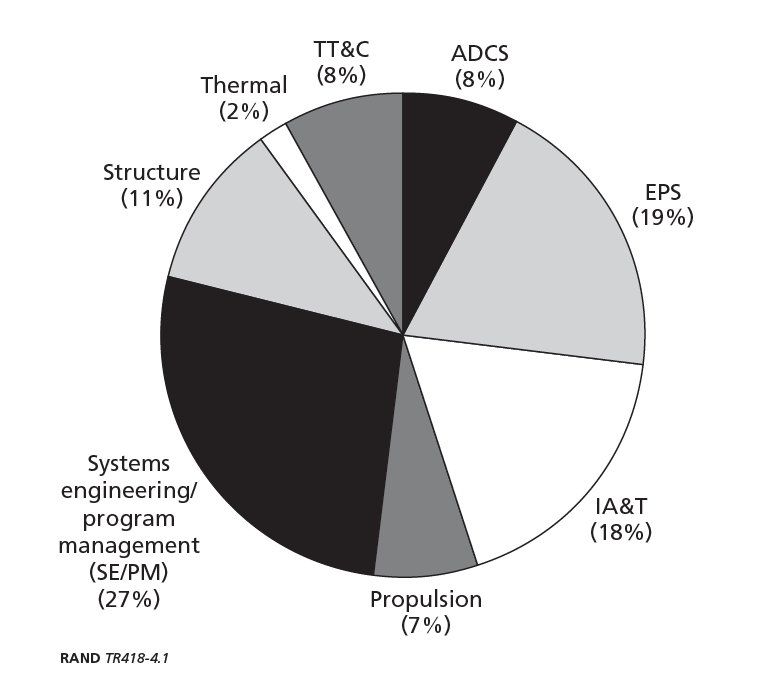
\includegraphics[width = .7\textwidth]{Torta.png}
			\caption{Communication spacecraft cost composition}
			\label{fig:torta}
		\end{figure}
		
		\begin{figure}
			\centering
			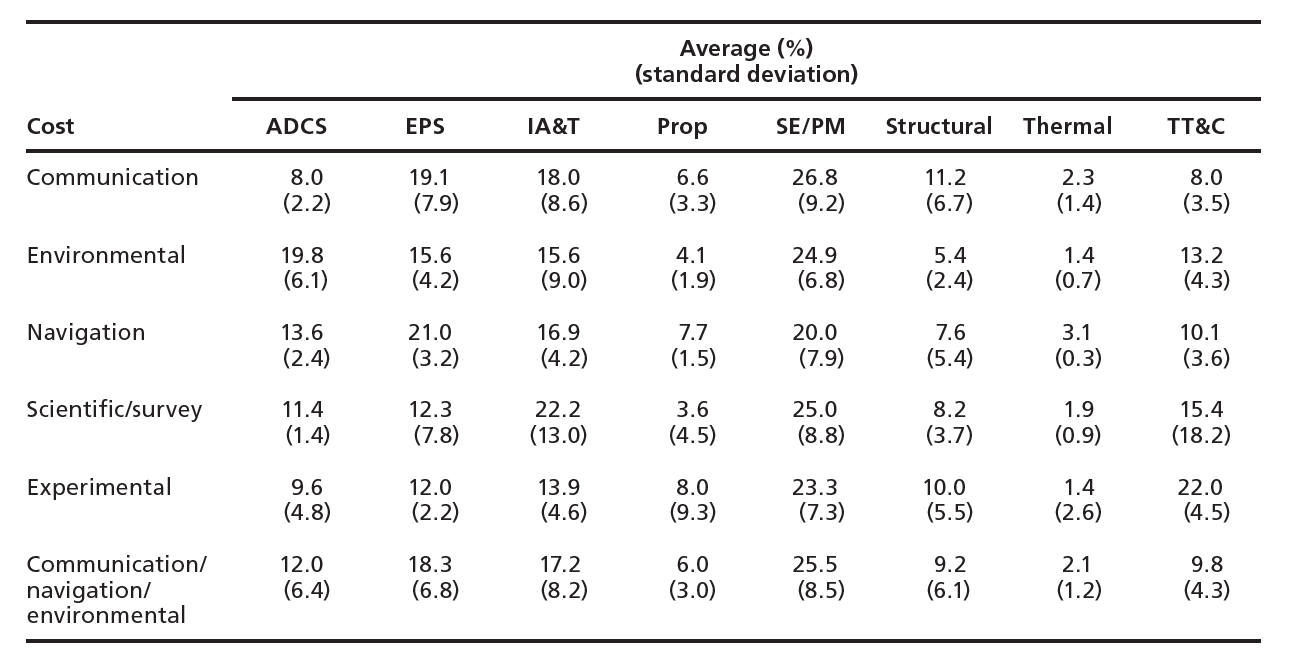
\includegraphics[width = 1\textwidth]{Standard_dev.png}
			\caption{Communication spacecraft cost composition: averages and standard deviations}
			\label{fig:distribution}
		\end{figure}
		
		\begin{figure}
			\centering
			\begin{minipage}{1\textwidth}
			\centering
			\includegraphics[width = .95\textwidth]{mission.png}
			\caption{Total spacecraft cost}
			\label{fig:mission}
			\end{minipage}
			\hspace{20mm}
			\begin{minipage}{.95\textwidth}
			\centering
			\includegraphics[width = .95\textwidth]{mission_pound.png}
			\caption{Total spacecraft cost per pound}
			\label{fig:mission_pound}
			\end{minipage}
		\end{figure}
		
		Regarding the cost per subsystem, \autoref{tab:systems1} and \autoref{tab:systems2} show the different cost each 				subsystem is intended to have:
		
		\begin{table}
			\centering
			\begin{tabular}{ccc}
			\toprule
			Subsystem & Mean Cost (k\euro) & Standard deviation\\
			\midrule
			IA\&T     & 8311,49   & 8719,94\\
			EPS        & 8441,34   & 5681,80\\
			Structure & 4111,49   & 2955,92\\
			SEPM      & 12167,05 & 7825,63\\
			Thermal  & 903,45    & 562,3\\
			TT\&C    & 4423,24   & 2942,24\\ 
			\bottomrule
			\end{tabular}
			\caption{List of the costs per subsystem}
			\label{tab:systems1}
		\end{table}
		
		\begin{table}
			\centering
			\begin{tabular}{ccc}
			\toprule
			Subsystem & Mean Cost/unit (k\euro/kg or ch) & Standard deviation\\
			\midrule
			ADCS                                         & 94,70     & 8719,94\\
			Communication ($1 < ch < 10$)   & 3923,19 & 1443,98\\
			Communication ($10 < ch < 25$) & 1534,45 & 558,37\\
			Communication ($25 < ch$)         & 708,40   & 197,35\\
			EPS                                            & 24,7      & 7,27\\
			Propulsion                                  & 54,68     & 14,32\\
			Structure                                    & 15,94     & 4,37\\
			\bottomrule
			\end{tabular}
			\caption{List of the costs per subsystem per pound/channel}
			\label{tab:systems2}
		\end{table}
		
		Through this data we can make a raw hypothesis on the average total cost of the spacecraft with a summary estimation 			of its mass:
		
		\begin{table}
			\centering
			\begin{tabular}{ccc}
			\toprule
			\multicolumn{3}{c}{Communication spacecraft}\\
			\midrule
			IA\&T       & 8311,49 \euro       & $+$\\
			EPS          & 24,7 \euro/Kg        & $\times NCHILI +$\\
			Structure   & 15,94  \euro/Kg     & $\times NCHILI +$\\
			SEPM        & 12167,05 \euro     & $+$\\
			Thermal    & 903,45 \euro        & $+$\\
			TT\&C       & 4423,24 \euro      & $+$\\ 
			ADCS        & 94,70 \euro/Kg     & $\times NCHILI +$\\
			Propulsion & 54,68   \euro/Kg   & $\times NCHILI +$\\
			Communication ($10 < ch < 25$) & 1534,45 \euro/ch & $\times 12 ch =$\\
			\bottomrule
			Total cost:& & TOT\\
			\end{tabular}
			\caption{List of the costs per subsystem per pound/channel}
			\label{tab:cost}
		\end{table}
	\subsection{Launch cost}
For the launch cost we based our considerations on the prices listed by the $SpaceX$ company. \autoref{fig:spacex} shows the prices for different types of launches, depending on the mass of the spacecrafts and the orbits they should reach.

Through the considerations we have made in the previous sections we can state that around $180$ Millions of dollars ($151.793.055$ \euro \cri{verifica il prezzo}) are needed for the launch: in fact each spacecraft has a total mass of about \cri{mettere massa} and the Molniya orbit is a HEO orbit; moreover, since the raans of the two orbital planes are separated of 180 $\deg$ it is necessary to use two separate launchers, one for each spacecraft.\\

Through this analysis the total cost for the project is:
\begin{equation}
Cost_{Total} = Cost_{Launch} + Cost_{Spacecraft} = \cri{Mettere costo finale} \text{\euro}
\end{equation}

\begin{figure}
\centering
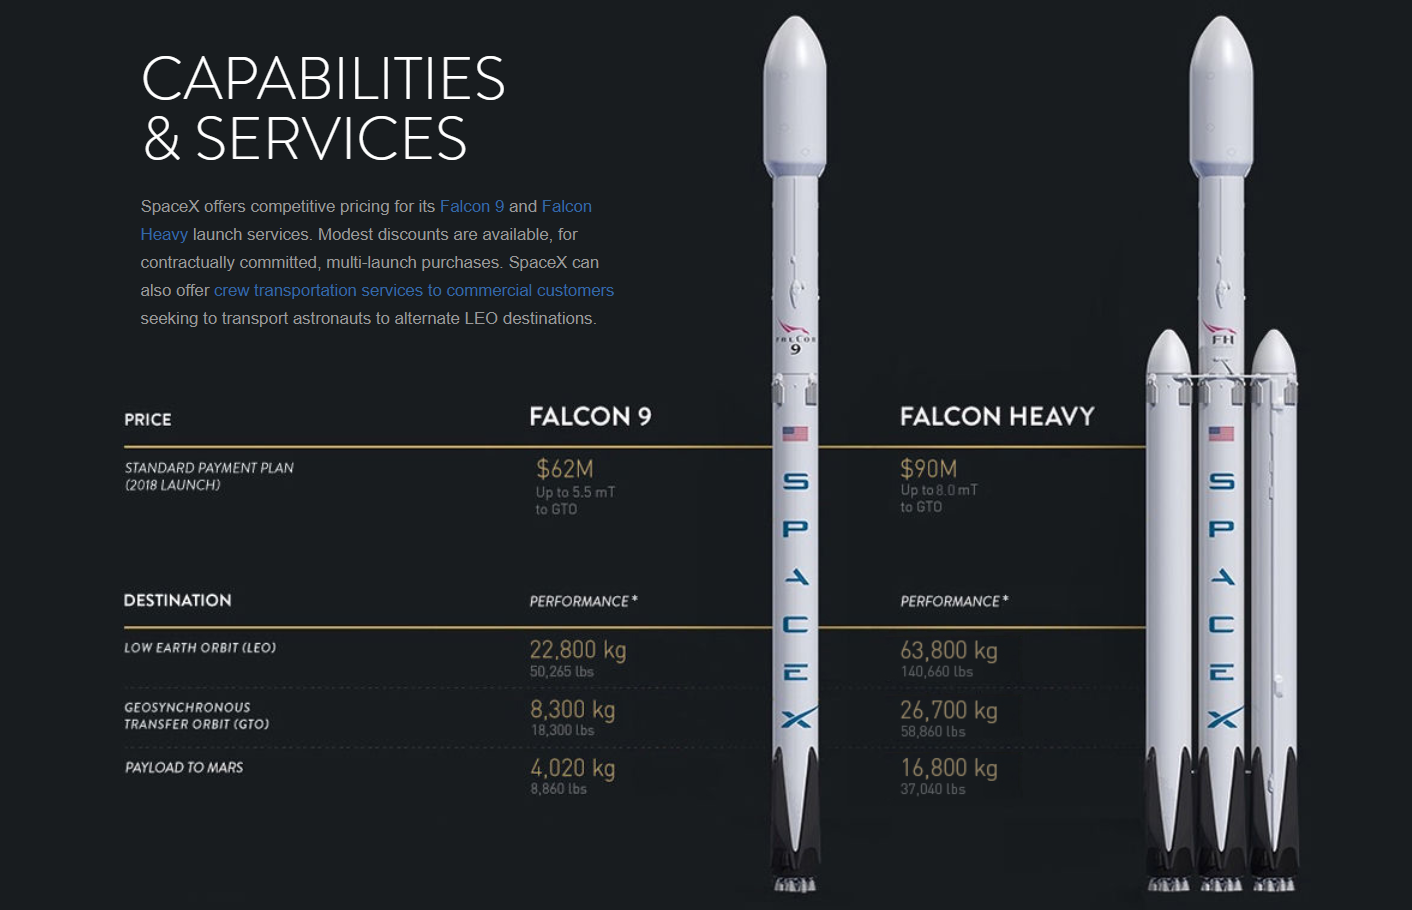
\includegraphics[width = .9\textwidth]{Spacex.png}
\caption{$SpaceX$ price list}
\label{fig:spacex}
\end{figure}

\section{Final considerations and conclusion}
\lipsum[1]























\end{document}
